\documentclass[11pt]{article}
\usepackage{amsmath, amssymb, physics, mathtools, bm}
\usepackage{tikz, pgfplots}
\pgfplotsset{compat=1.18}
\usetikzlibrary{decorations.pathmorphing, arrows.meta, calc}
\usepackage[margin=2.3cm]{geometry}
\usepackage{siunitx, booktabs, hyperref}
\usepackage{braket}

\newcommand{\D}{\mathrm{D}}
\newcommand{\de}{\mathrm{d}}
\newcommand{\pd}[2]{\frac{\partial #1}{\partial #2}}
\newcommand{\pdd}[2]{\frac{\partial^{2} #1}{\partial #2^{2}}}
\newcommand{\Lap}{\nabla^{2}}

\title{B1 Fluids --- Model Solutions, MT 2020}
\author{}
\date{}

\begin{document}
\maketitle

%==================================================================
\section*{Question 1 --- Oscillating plate (Stokes' second problem)}

\textbf{Problem.} Incompressible viscous fluid above an infinite plate at $z=0$ that oscillates as $\vb u|_{z=0}=(U\cos\omega t,0)$; velocity decays for $z\to\infty$. Gravity neglected.

\subsection*{(a) Governing equations}

Incompressible Navier--Stokes (no gravity):
\begin{equation}
\pd{\vb u}{t}+(\vb u\cdot\nabla)\vb u=-\frac{1}{\rho}\nabla p+\nu\Lap\vb u.
\label{eq:NS}
\end{equation}
Mass conservation:
\[
\nabla\cdot\vb u=0.
\]
Term-by-term: $\partial_t\vb u$ local acceleration; $(\vb u\cdot\nabla)\vb u$ advective (inertial) acceleration; $-\rho^{-1}\nabla p$ pressure-gradient force; $\nu\Lap\vb u$ viscous diffusion of momentum; $\nabla\cdot\vb u=0$ enforces incompressibility.

\subsection*{(b) Velocity field}

Translation invariance: plate is infinite in $x$, forcing is $x$-independent:
\[
\vb u=[u_x(z,t),u_z(z,t)],\qquad p=p(z,t).
\]
Mass conservation:
\[
\pd{u_z}{z}=0.
\]
Apply $u_z\to 0$ as $z\to\infty$:
\[
u_z\equiv 0.
\]
Substitute into $x$-component of \eqref{eq:NS} (advection $u_z\partial_z u_x=0$, no $\partial_x p$):
\begin{equation}
\pd{u_x}{t}=\nu\pdd{u_x}{z}.
\label{eq:diffux}
\end{equation}
Try $u_x=\Re[u_0(z)e^{i\omega t}]$:
\[
i\omega u_0=\nu u_0''.
\]
Rearrange:
\[
u_0''=\frac{i\omega}{\nu}u_0.
\]
Characteristic roots $\pm k$ with $k^2=i\omega/\nu$:
\[
k=\sqrt{i\omega/\nu}.
\]
Apply $\sqrt{i}=(1+i)/\sqrt{2}$:
\[
k=(1+i)\sqrt{\omega/(2\nu)}.
\]
Define $\delta=\sqrt{2\nu/\omega}$:
\[
k=\frac{1+i}{\delta}.
\]
Decay as $z\to\infty$ kills $e^{+kz}$:
\[
u_0(z)=U e^{-kz}.
\]
Apply $u_x(0,t)=U\cos\omega t$, fixing the amplitude $U$ real:
\[
u_x(z,t)=\Re\!\left[U e^{-(1+i)z/\delta}e^{i\omega t}\right].
\]
Combine exponentials in the bracket:
\[
u_x(z,t)=\Re\!\left[U e^{-z/\delta}e^{i(\omega t-z/\delta)}\right].
\]
Take the real part:
\begin{equation}
\boxed{\;u_x(z,t)=U e^{-z/\delta}\cos\!\left(\omega t-\frac{z}{\delta}\right),\qquad u_z=0\;}
\label{eq:ux}
\end{equation}

\subsection*{(c) Stress tensor}

Newtonian stress:
\[
\sigma_{ij}=-p\,\delta_{ij}+\mu\!\left(\pd{u_i}{x_j}+\pd{u_j}{x_i}\right).
\]
Use $u_z=0$ and $\partial_x u_x=0$:
\[
\sigma_{xx}=-p,\qquad \sigma_{zz}=-p.
\]
Off-diagonal:
\[
\sigma_{xz}=\sigma_{zx}=\mu\pd{u_x}{z}.
\]
Differentiate the exponential prefactor:
\[
\pd{}{z}\!\left[Ue^{-z/\delta}\right]=-\frac{U}{\delta}e^{-z/\delta}.
\]
Differentiate the phase using $\partial_z\cos(\omega t-z/\delta)=(1/\delta)\sin(\omega t-z/\delta)$:
\[
\pd{u_x}{z}=-\frac{U}{\delta}e^{-z/\delta}\cos\!\left(\omega t-\tfrac{z}{\delta}\right)+\frac{U}{\delta}e^{-z/\delta}\sin\!\left(\omega t-\tfrac{z}{\delta}\right).
\]
Factor $-Ue^{-z/\delta}/\delta$:
\[
\pd{u_x}{z}=-\frac{U}{\delta}e^{-z/\delta}\!\left[\cos\!\left(\omega t-\tfrac{z}{\delta}\right)-\sin\!\left(\omega t-\tfrac{z}{\delta}\right)\right].
\]
Apply $\cos\alpha-\sin\alpha=\sqrt 2\cos(\alpha+\pi/4)$:
\[
\pd{u_x}{z}=-\frac{\sqrt 2\,U}{\delta}e^{-z/\delta}\cos\!\left(\omega t-\frac{z}{\delta}+\frac{\pi}{4}\right).
\]
Therefore
\[
\boxed{\;\sigma_{xz}=\sigma_{zx}=-\mu\frac{\sqrt 2\,U}{\delta}e^{-z/\delta}\cos\!\left(\omega t-\frac{z}{\delta}+\frac{\pi}{4}\right),\qquad \sigma_{xx}=\sigma_{zz}=-p\;}
\]
($p$ undetermined to within an additive constant since $\partial_z p=0$ and gravity is neglected).

\subsection*{(d) Profiles, force balance, boundary layer}

Profiles:
\[
u_x(z,t=2n\pi/\omega)=Ue^{-z/\delta}\cos(z/\delta),\qquad u_x(z,t=(2n+\tfrac12)\pi/\omega)=Ue^{-z/\delta}\sin(z/\delta).
\]

\begin{center}
\begin{tikzpicture}[>=stealth, scale=1.0]
  \draw[->] (-2.5,0) -- (3.5,0) node[right] {$u_x/U$};
  \draw[->] (0,0) -- (0,5.5) node[above] {$z/\delta$};
  \draw (1,0.06) -- (1,-0.06) node[below] {\small $1$};
  \draw (-1,0.06) -- (-1,-0.06) node[below] {\small $-1$};
  \draw[thick,blue,domain=0:5,samples=80,smooth,variable=\z]
      plot ({exp(-\z)*cos(\z)},{\z});
  \draw[thick,red,dashed,domain=0:5,samples=80,smooth,variable=\z]
      plot ({exp(-\z)*sin(\z)},{\z});
  \node[circle,fill,inner sep=1.2pt] (P) at (1,0) {};
  \node[below right] at (P) {\small plate};
  \node[blue,right] at (0.95,0.55) {\small $\omega t=2n\pi$};
  \node[red, right] at (0.65,1.9) {\small $\omega t=(2n+\tfrac12)\pi$};
  \draw[<->,gray] (-2.0,0) -- (-2.0,1) node[midway,left]{\small $\delta$};
  \draw[gray,dashed] (-2.0,1) -- (0,1);
\end{tikzpicture}
\end{center}

Force balance: in \eqref{eq:diffux} unsteady inertia $\partial_t u_x$ balances viscous diffusion $\nu\partial_z^2 u_x$. Pressure is uniform; advection vanishes. Momentum injected at the plate diffuses upward while the imposed phase reverses every half period, generating the damped travelling wave \eqref{eq:ux}.

Boundary-layer thickness from $\delta=\sqrt{2\nu/\omega}$:
\[
\boxed{\;\delta=\sqrt{2\nu/\omega}\;}
\]
Independent of $U$. Physical reading: in one forcing period $T=2\pi/\omega$ vorticity diffuses a distance $\sqrt{\nu T}\sim\delta$ before the surface reverses, halting further penetration.

Tidal-flow application: by Galilean change of frame to one in which the fluid oscillates at $-U\cos\omega t$ and the plate is fixed, the same equation governs flow over a stationary bed with oscillatory far-field velocity. So an oscillatory Stokes layer of thickness $\delta=\sqrt{2\nu/\omega}$ does form near a tidal bed. Numerical estimate ($\nu=\SI{e-6}{m^2.s^{-1}}$, $\omega=\SI{1.4e-4}{s^{-1}}$ semi-diurnal): $\delta\sim\SI{10}{cm}$. Caveats: real tidal flow is turbulent (large $\mathrm{Re}$), so the laminar Stokes layer is replaced by a thicker turbulent boundary layer; the laminar solution describes only the viscous sub-layer.

%==================================================================
\section*{Question 2 --- Active cylinder, potential flow}

\textbf{Problem.} 2D inviscid, incompressible, irrotational flow past cylinder $r=a$ with prescribed normal velocity $u_r(a,\theta)=A\sin\theta$, far-field $\vb u\to-U\hat{\vb x}$, $p\to p_0$. Cylinder axis vertical.

\subsection*{(a) Velocity potential and Bernoulli}

Irrotational: $\nabla\times\vb u=0$, so $\vb u=\nabla\phi$. Incompressible: $\nabla\cdot\vb u=0$, hence
\[
\Lap\phi=0.
\]
Euler with gravity:
\[
\pd{\vb u}{t}+(\vb u\cdot\nabla)\vb u=-\frac{1}{\rho}\nabla p-g\hat{\vb z}.
\]
Vector identity:
\[
(\vb u\cdot\nabla)\vb u=\nabla(\tfrac12 |\vb u|^2)-\vb u\times(\nabla\times\vb u).
\]
Apply $\nabla\times\vb u=0$:
\[
(\vb u\cdot\nabla)\vb u=\nabla(\tfrac12|\vb u|^2).
\]
Apply $\vb u=\nabla\phi$ in the local-acceleration term:
\[
\pd{\vb u}{t}=\pd{}{t}\nabla\phi=\nabla\!\left(\pd{\phi}{t}\right).
\]
Write $-g\hat{\vb z}=-\nabla(gz)$ and $-\nabla p/\rho=-\nabla(p/\rho)$ (constant $\rho$):
\[
\nabla\!\left(\pd{\phi}{t}+\tfrac12|\nabla\phi|^2+\frac{p}{\rho}+gz\right)=0.
\]
Therefore $\nabla H=0$ with
\begin{equation}
\boxed{\;H=\pd{\phi}{t}+\tfrac12|\vb u|^2+\frac{p}{\rho}+gz\;}
\label{eq:bernoulli}
\end{equation}
Steady interpretation: $\partial_t\phi=0$, so $H$ is the conserved total mechanical energy per unit mass --- kinetic + pressure-work term + gravitational potential.

\subsection*{(b) Solution and surface pressure}

BCs:
\[
\pd{\phi}{r}\bigg|_{r=a}=A\sin\theta,\qquad \nabla\phi\to-U\hat{\vb x}\text{ as }r\to\infty.
\]
Resolve $-U\hat{\vb x}=-U\cos\theta\,\hat{\vb r}+U\sin\theta\,\hat{\bm\theta}$:
\[
\phi\to -Ur\cos\theta\quad (r\to\infty).
\]
From the general expansion keep $n=1$ modes only (BCs only excite $\sin\theta,\cos\theta$):
\[
\phi=\left(A_1 r+\frac{B_1}{r}\right)\cos\theta+\left(C_1 r+\frac{D_1}{r}\right)\sin\theta.
\]
Take $r\to\infty$, where $B_1/r,D_1/r\to 0$:
\[
\phi\to A_1 r\cos\theta+C_1 r\sin\theta.
\]
Match to $-Ur\cos\theta$:
\[
A_1=-U,\qquad C_1=0.
\]
Differentiate $\phi$ in $r$:
\[
\pd{\phi}{r}=\left(A_1-\frac{B_1}{r^2}\right)\cos\theta+\left(C_1-\frac{D_1}{r^2}\right)\sin\theta.
\]
Evaluate at $r=a$ with $A_1=-U,C_1=0$:
\[
\left(-U-\frac{B_1}{a^2}\right)\cos\theta+\left(-\frac{D_1}{a^2}\right)\sin\theta=A\sin\theta.
\]
Match coefficients:
\[
B_1=-Ua^2,\qquad D_1=-Aa^2.
\]
Hence
\begin{equation}
\boxed{\;\phi(r,\theta)=-U\!\left(r+\frac{a^2}{r}\right)\cos\theta-\frac{Aa^2}{r}\sin\theta\;}
\label{eq:phi-cyl}
\end{equation}
Velocity:
\[
u_r=\pd{\phi}{r}=-U\!\left(1-\frac{a^2}{r^2}\right)\cos\theta+\frac{Aa^2}{r^2}\sin\theta,
\]
\[
u_\theta=\frac{1}{r}\pd{\phi}{\theta}=U\!\left(1+\frac{a^2}{r^2}\right)\sin\theta-\frac{Aa^2}{r^2}\cos\theta.
\]
At $r=a$:
\[
u_r(a,\theta)=A\sin\theta,\qquad u_\theta(a,\theta)=2U\sin\theta-A\cos\theta.
\]
Surface speed squared:
\[
|\vb u(a,\theta)|^2=A^2\sin^2\theta+(2U\sin\theta-A\cos\theta)^2.
\]
Expand the square:
\[
(2U\sin\theta-A\cos\theta)^2=4U^2\sin^2\theta-4UA\sin\theta\cos\theta+A^2\cos^2\theta.
\]
Insert into $|\vb u|^2$:
\[
|\vb u|^2=A^2\sin^2\theta+4U^2\sin^2\theta-4UA\sin\theta\cos\theta+A^2\cos^2\theta.
\]
Apply $\sin^2\theta+\cos^2\theta=1$ to combine the $A^2$ terms:
\[
|\vb u|^2=A^2+4U^2\sin^2\theta-4UA\sin\theta\cos\theta.
\]
Apply $2\sin\theta\cos\theta=\sin 2\theta$:
\[
|\vb u|^2=A^2+4U^2\sin^2\theta-2UA\sin 2\theta.
\]
Apply steady Bernoulli between far-field and the cylinder surface (same horizontal level, $gz$ cancels):
\[
p_0+\tfrac12\rho U^2=p(a,\theta)+\tfrac12\rho|\vb u(a,\theta)|^2.
\]
Solve for $p(a,\theta)$:
\[
p(a,\theta)=p_0+\tfrac12\rho U^2-\tfrac12\rho\!\left[A^2+4U^2\sin^2\theta-2UA\sin 2\theta\right].
\]
Apply $\sin^2\theta=\tfrac12(1-\cos 2\theta)$ to $4U^2\sin^2\theta$:
\[
4U^2\sin^2\theta=2U^2-2U^2\cos 2\theta.
\]
Substitute into $-\tfrac12\rho[A^2+4U^2\sin^2\theta-2UA\sin 2\theta]$:
\[
-\tfrac12\rho[\,\cdots\,]=-\tfrac12\rho A^2-\rho U^2+\rho U^2\cos 2\theta+\rho UA\sin 2\theta.
\]
Add the $p_0+\tfrac12\rho U^2$ outside:
\[
p(a,\theta)=p_0+\tfrac12\rho U^2-\tfrac12\rho A^2-\rho U^2+\rho U^2\cos 2\theta+\rho UA\sin 2\theta.
\]
Combine $\tfrac12\rho U^2-\rho U^2=-\tfrac12\rho U^2$:
\[
p(a,\theta)=p_0-\tfrac12\rho U^2-\tfrac12\rho A^2+\rho U^2\cos 2\theta+\rho UA\sin 2\theta.
\]
Factor $\tfrac12\rho U^2$:
\begin{equation}
\boxed{\;p(a,\theta)=p_0+\tfrac12\rho U^2\!\left[2\cos 2\theta-1-\frac{A^2}{U^2}+2\frac{A}{U}\sin 2\theta\right]\;}
\label{eq:psurf}
\end{equation}

Sketch of $\Delta p\equiv p(a,\theta)-p_0$ in units of $\tfrac12\rho U^2$:

\begin{center}
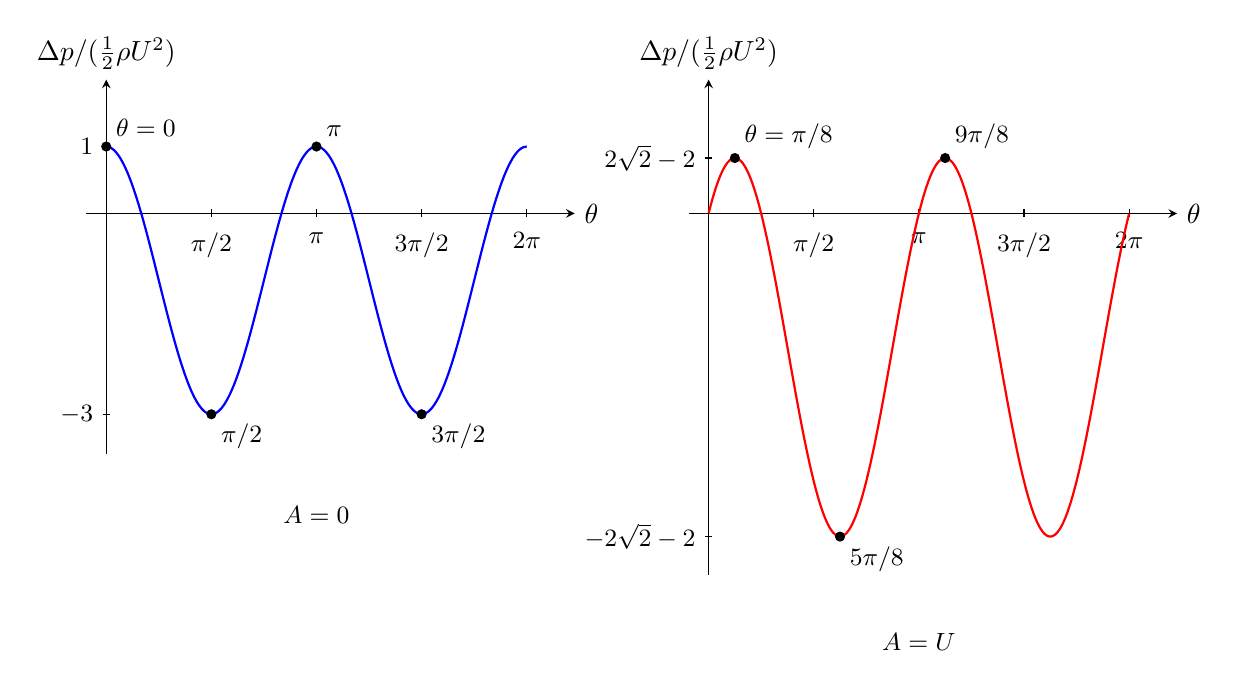
\begin{tikzpicture}[>=stealth, scale=0.85]
  % --- A=0 panel ---
  \begin{scope}
    \draw[->] (-0.3,0) -- (7,0) node[right] {$\theta$};
    \draw[->] (0,-3.6) -- (0,2.0) node[above] {$\Delta p/(\tfrac12\rho U^2)$};
    \foreach \x/\lab in {1.5708/{\pi/2},3.1416/{\pi},4.7124/{3\pi/2},6.2832/{2\pi}}
       \draw (\x,0.06) -- (\x,-0.06) node[below=2pt] {\small $\lab$};
    \draw (0.05,1) -- (-0.05,1) node[left] {\small $1$};
    \draw (0.05,-3) -- (-0.05,-3) node[left] {\small $-3$};
    \draw[thick,blue,domain=0:6.2832,samples=120,smooth]
        plot (\x,{2*cos(2*\x r) - 1});
    \node[circle,fill,inner sep=1.3pt] (M0) at (0,1) {};
    \node[above right] at (M0) {\small $\theta=0$};
    \node[circle,fill,inner sep=1.3pt] (M1) at (1.5708,-3) {};
    \node[below right] at (M1) {\small $\pi/2$};
    \node[circle,fill,inner sep=1.3pt] (M2) at (3.1416,1) {};
    \node[above right] at (M2) {\small $\pi$};
    \node[circle,fill,inner sep=1.3pt] (M3) at (4.7124,-3) {};
    \node[below right] at (M3) {\small $3\pi/2$};
    \node at (3.1416,-4.5) {\small $A=0$};
  \end{scope}
  % --- A=U panel ---
  \begin{scope}[xshift=9cm]
    \draw[->] (-0.3,0) -- (7,0) node[right] {$\theta$};
    \draw[->] (0,-5.4) -- (0,2.0) node[above] {$\Delta p/(\tfrac12\rho U^2)$};
    \foreach \x/\lab in {1.5708/{\pi/2},3.1416/{\pi},4.7124/{3\pi/2},6.2832/{2\pi}}
       \draw (\x,0.06) -- (\x,-0.06) node[below=2pt] {\small $\lab$};
    \draw (0.05,0.828) -- (-0.05,0.828) node[left] {\small $2\sqrt 2-2$};
    \draw (0.05,-4.828) -- (-0.05,-4.828) node[left] {\small $-2\sqrt 2-2$};
    \draw[thick,red,domain=0:6.2832,samples=160,smooth]
        plot (\x,{2*cos(2*\x r) - 2 + 2*sin(2*\x r)});
    \node[circle,fill,inner sep=1.3pt] (P1) at (0.3927,0.828) {};
    \node[above right] at (P1) {\small $\theta=\pi/8$};
    \node[circle,fill,inner sep=1.3pt] (P2) at (1.9635,-4.828) {};
    \node[below right] at (P2) {\small $5\pi/8$};
    \node[circle,fill,inner sep=1.3pt] (P3) at (3.5343,0.828) {};
    \node[above right] at (P3) {\small $9\pi/8$};
    \node at (3.1416,-6.4) {\small $A=U$};
  \end{scope}
\end{tikzpicture}
\end{center}

For $A=0$, fore--aft symmetric about $\theta=\pi/2,3\pi/2$; for $A=U$, the curve shifts and tilts: maximum suction at $\theta=5\pi/8$, peak pressure at $\theta=\pi/8$ --- a transverse asymmetry that lifts the cylinder.

\subsection*{(c) Boundary-layer separation}

Inert case $A=0$. Inviscid surface speed $u_\theta=2U\sin\theta$, so a no-slip boundary layer grows everywhere except the stagnation points $\theta=0,\pi$. Surface pressure gradient (using \eqref{eq:psurf} with $A=0$):
\[
\frac{1}{a}\pd{p}{\theta}=-\frac{2\rho U^2}{a}\sin 2\theta.
\]
Adverse on the rear half, $\pi/2<\theta<\pi$ (and mirror $\pi<\theta<3\pi/2$). Separation occurs shortly after $\theta=\pi/2$ on top and shortly after $\theta=3\pi/2$ on the bottom (rear shoulders).

Active case $A=U$, upper surface $0<\theta<\pi$. Differentiate \eqref{eq:psurf}:
\[
\frac{1}{a}\pd{p}{\theta}=\frac{\rho U^2}{a}\!\left[-2\sin 2\theta+2\cos 2\theta\right].
\]
Locate the surface pressure extrema by $\partial_\theta p=0$:
\[
\tan 2\theta=1\;\Rightarrow\;\theta=\pi/8\;\text{(maximum)},\;\theta=5\pi/8\;\text{(minimum)}.
\]
Inviscid surface tangential velocity $u_\theta(a,\theta)=2U\sin\theta-U\cos\theta$, vanishing at the shifted stagnation $\tan\theta=1/2$ ($\theta\approx 0.46$). Downstream of that stagnation on $\theta>0$, flow runs in $+\theta$ and pressure minimum is reached at $\theta=5\pi/8$; adverse region is $5\pi/8<\theta<\pi$. Compared with $A=0$ (adverse from $\theta=\pi/2$) the adverse-pressure region starts later, pushing the would-be separation point further back. The imposed $u_r=A\sin\theta>0$ also blows fluid \emph{outward} from the wall on $\theta>0$, energising the boundary layer (analogous to suction--blowing control). Both effects \emph{inhibit} separation on the upper surface relative to $A=0$.

%==================================================================
\section*{Question 3 --- Vorticity dynamics and shear-layer mode}

\textbf{Problem.} Vorticity equation, piecewise-shear base flow, linear interfacial mode.

\subsection*{(a) Vorticity equation}

Take curl of incompressible Navier--Stokes:
\[
\pd{\bm\omega}{t}+\nabla\times[(\vb u\cdot\nabla)\vb u]=\nu\Lap\bm\omega.
\]
Identity:
\[
(\vb u\cdot\nabla)\vb u=\nabla(\tfrac12|\vb u|^2)-\vb u\times\bm\omega.
\]
Take curl, use $\nabla\times\nabla(\cdot)=0$ and $\nabla\cdot\vb u=\nabla\cdot\bm\omega=0$:
\[
\nabla\times(\vb u\times\bm\omega)=(\bm\omega\cdot\nabla)\vb u-(\vb u\cdot\nabla)\bm\omega.
\]
Combine:
\begin{equation}
\boxed{\;\frac{\D\bm\omega}{\D t}=(\bm\omega\cdot\nabla)\vb u+\nu\Lap\bm\omega\;}
\label{eq:vort}
\end{equation}
Term-by-term: $\D\bm\omega/\D t$ material rate of vorticity change following a fluid parcel; $(\bm\omega\cdot\nabla)\vb u$ vortex stretching/tilting by the velocity gradient; $\nu\Lap\bm\omega$ viscous diffusion of vorticity.

2D inviscid: $\bm\omega=\omega_z(x,y,t)\hat{\vb z}$, no $z$-gradients in $\vb u$:
\[
(\bm\omega\cdot\nabla)\vb u=\omega_z\partial_z\vb u=0.
\]
Drop viscosity:
\[
\frac{\D\omega_z}{\D t}=0.
\]
Streamfunction: $u_x=\partial_y\psi$, $u_y=-\partial_x\psi$, so $\omega_z=\partial_x u_y-\partial_y u_x=-\Lap\psi$:
\begin{equation}
\frac{\D}{\D t}\Lap\psi=0.
\label{eq:psi-vort}
\end{equation}

\subsection*{(b) Base flow}

From $\overline U=\partial_y\overline\psi$:
\[
\overline\psi(y)=\int_0^y\overline U(y')\,\de y'.
\]
Piecewise integration:
\[
\overline\psi(y)=\begin{cases}-\tfrac12\alpha y^2,& y\ge 0,\\ 0,& y<0.\end{cases}
\]
Vorticity $\overline\omega_z=-\partial_y^2\overline\psi$:
\[
\boxed{\;\overline\omega_z(y)=\begin{cases}\alpha,& y>0,\\ 0,& y<0.\end{cases}\;}
\]
Each layer has uniform $\overline\omega_z$, and the base flow is steady and parallel: $\D(\Lap\overline\psi)/\D t=\overline U\partial_x(\Lap\overline\psi)=0$, satisfying \eqref{eq:psi-vort}.

\subsection*{(c) Linearised mode}

Total $\psi=\overline\psi(y)+\Re[\hat\psi(y)e^{ikx-i\omega t}]$. Linearise \eqref{eq:psi-vort}:
\[
\left(\pd{}{t}+\overline U\pd{}{x}\right)\Lap\psi'-(\Lap\overline\psi)_{,y}\,\pd{\psi'}{x}=0.
\]
Within each layer $\overline U''=0$, so:
\[
(-i\omega+ik\overline U)(-k^2\hat\psi+\hat\psi'')=0.
\]
Cancel $\omega-k\overline U\ne 0$:
\begin{equation}
\boxed{\;\hat\psi''-k^2\hat\psi=0\;}
\label{eq:psihat-ode}
\end{equation}
Solutions decaying as $|y|\to\infty$ (take $k>0$):
\[
\hat\psi(y)=\begin{cases}C_+ e^{-ky},& y>0,\\ C_- e^{+ky},& y<0.\end{cases}
\]

Pressure from horizontal momentum (linearised, $u_x'=\partial_y\psi'$, $u_y'=-\partial_x\psi'$):
\[
\pd{u_x'}{t}+\overline U\pd{u_x'}{x}+u_y'\pd{\overline U}{y}=-\frac{1}{\rho}\pd{p'}{x}.
\]
Substitute mode form $u_x'=\hat\psi' e^{i(kx-\omega t)}$, $u_y'=-ik\hat\psi e^{i(kx-\omega t)}$:
\[
(-i\omega+ik\overline U)\hat\psi'+(-ik\hat\psi)\,\overline U'=-\frac{ik}{\rho}\hat p.
\]
Factor $i$ on the left:
\[
i(k\overline U-\omega)\hat\psi'-ik\hat\psi\,\overline U'=-\frac{ik}{\rho}\hat p.
\]
Divide both sides by $-ik$:
\[
\frac{\omega-k\overline U}{k}\hat\psi'+\hat\psi\,\overline U'=\frac{\hat p}{\rho}.
\]
Solve for $\hat p$:
\begin{equation}
\boxed{\;\hat p=\rho\!\left[\frac{\omega-k\overline U}{k}\,\pd{\hat\psi}{y}+\hat\psi\,\pd{\overline U}{y}\right]\;}
\label{eq:phat}
\end{equation}

Interface matching at $y=\eta$. Continuity of normal velocity / displacement gives $[\hat\psi]_-^+=0$ at $y=0$. Continuity of pressure (no surface tension) gives, using \eqref{eq:phat} at $\overline U(0)=0$:
\[
\left[\frac{\omega}{k}\pd{\hat\psi}{y}+\hat\psi\,\pd{\overline U}{y}\right]_-^+=0\quad\text{at }y=0.
\]

Apply continuity of $\hat\psi$ at $y=0$:
\[
C_+=C_-\equiv C.
\]
Differentiate the layer solutions:
\[
\hat\psi'(0^+)=-kC,\qquad \hat\psi'(0^-)=+kC.
\]
Read off base shear from $\overline U(y)=-\alpha y\,(y>0)$, $\overline U(y)=0\,(y<0)$:
\[
\overline U'(0^+)=-\alpha,\qquad \overline U'(0^-)=0.
\]
Insert into the second matching condition:
\[
\left[\frac{\omega}{k}(-kC)+C(-\alpha)\right]-\left[\frac{\omega}{k}(+kC)+C(0)\right]=0.
\]
Expand:
\[
-\omega C-\alpha C-\omega C=0.
\]
Collect:
\[
-2\omega C-\alpha C=0.
\]
Factor $C\ne 0$ and solve for $\omega$:
\begin{equation}
\boxed{\;\omega=-\frac{\alpha}{2}\;}
\label{eq:omega-result}
\end{equation}

Streamfunction (to within multiplicative constant):
\[
\boxed{\;\hat\psi(y)=C\,e^{-k|y|}\;}
\]

Evolution. $\omega$ is real $\Rightarrow$ disturbance is neutrally stable: amplitude constant in time. Phase factor $e^{ikx-i\omega t}=e^{ik(x+\alpha t/(2k))}$, giving phase speed $c=\omega/k=-\alpha/(2k)$ in $\hat{\vb x}$ (wave travels in $-x$ for $\alpha>0$). Spatial structure: $\hat\psi\propto e^{-k|y|}$, decays exponentially away from the interface --- a localised vorticity-edge wave on the kink in $\overline U(y)$.

%==================================================================
\section*{Question 4 --- Lubrication: rotating cylinder near a plane}

\textbf{Problem.} Long rigid cylinder, axis $\parallel\hat{\vb y}$, radius $a$, rotating $\Omega\hat{\vb y}$ above plane $z=0$, immersed in incompressible viscous fluid.

\subsection*{(a) Reynolds number}

\[
\boxed{\;\mathrm{Re}=\frac{UL}{\nu}=\frac{\rho UL}{\mu}\;}
\]
ratio of inertial to viscous forces. High $\mathrm{Re}\gg 1$: inertia dominates, viscous effects confined to thin boundary layers and wakes; turbulence possible. Low $\mathrm{Re}\ll 1$ (Stokes flow): viscous balance, time-reversible, flow $\Lap\vb u=\nabla p/\mu$ linear in boundary forcing, no separation, no inertia.

\subsection*{(b)(i) Geometry, BCs, surface velocity}

Cylinder axis at $z=a+h_0$. Surface: $z_{\text{cyl}}=a+h_0-\sqrt{a^2-x^2}$. Gap height:
\[
h(x)=z_{\text{cyl}}(x)=h_0+a-\sqrt{a^2-x^2}.
\]
Binomial expand for $x\ll a$:
\[
\sqrt{a^2-x^2}=a\sqrt{1-x^2/a^2}\approx a-\frac{x^2}{2a}.
\]
Substitute:
\begin{equation}
\boxed{\;h(x)\approx h_0+\frac{x^2}{2a}\;}
\label{eq:h-paraboloid}
\end{equation}

Boundary conditions. No-slip + impermeability on rigid surfaces:
\[
\vb u(z=0)=\vb 0,\qquad \vb u\big|_{\text{cyl surface}}=\Omega\hat{\vb y}\times\vb r_{\text{from axis}}.
\]
Position of contact-region surface point relative to axis:
\[
\vb r_{\text{from axis}}=x\hat{\vb x}-(\sqrt{a^2-x^2})\hat{\vb z}.
\]
Apply $\hat{\vb y}\times\hat{\vb x}=-\hat{\vb z}$, $\hat{\vb y}\times\hat{\vb z}=\hat{\vb x}$:
\[
\Omega\hat{\vb y}\times\vb r_{\text{from axis}}=\Omega x(-\hat{\vb z})-\Omega\sqrt{a^2-x^2}\,\hat{\vb x}.
\]
Collect:
\[
\Omega\hat{\vb y}\times\vb r_{\text{from axis}}=-\Omega\sqrt{a^2-x^2}\,\hat{\vb x}-\Omega x\,\hat{\vb z}.
\]
Apply $x\ll a$ in $\sqrt{a^2-x^2}\approx a$:
\[
\Omega\hat{\vb y}\times\vb r_{\text{from axis}}\approx -\Omega a\,\hat{\vb x}-\Omega x\,\hat{\vb z}.
\]
Drop $\hat{\vb z}$-component as $O(\Omega x)\ll |\Omega a|$:
\[
\boxed{\;\vb u(x,z=h(x))\approx U\hat{\vb x},\qquad U=-\Omega a\;}
\]

\subsection*{(b)(ii) Lubrication equation}

Translation invariance: cylinder is long, $\partial_y\equiv 0$, $u_y\approx 0$. Aspect ratio $\epsilon\equiv h_0/a\ll 1$. From $\nabla\cdot\vb u=0$:
\[
u_z\sim \epsilon\,u_x.
\]
Compare derivatives:
\[
\pdd{u_x}{x}\sim u_x/a^2,\qquad \pdd{u_x}{z}\sim u_x/h_0^2,\qquad\text{ratio}=\epsilon^2\ll 1.
\]
Drop $\partial_x^2 u_x$. Reduced Reynolds number:
\[
\frac{\rho u_x \partial_x u_x}{\mu\,\partial_z^2 u_x}\sim \frac{\rho U^2/a}{\mu U/h_0^2}=\frac{\rho U h_0^2}{\mu a}=\mathrm{Re}\,\epsilon^2\ll 1.
\]
Drop inertia. Required: $h\ll a$ and $\rho U h^2/(\mu a)\ll 1$. The $x$-momentum equation reduces to
\begin{equation}
\boxed{\;\mu\pdd{u_x}{z}\approx -\pd{p}{x}\;}
\label{eq:lub}
\end{equation}

Neglect $\partial_x p$ as instructed:
\[
\pdd{u_x}{z}=0.
\]
Integrate twice in $z$:
\[
u_x(x,z)=B(x)z+C(x).
\]
Apply $u_x(z=0)=0$:
\[
C(x)=0.
\]
Apply $u_x(z=h)=U=-\Omega a$:
\[
B(x)=\frac{U}{h(x)}=-\frac{\Omega a}{h(x)}.
\]
Therefore
\begin{equation}
\boxed{\;u_x(x,z)\approx \frac{U\,z}{h(x)}=-\frac{\Omega a\,z}{h(x)}\;}
\label{eq:lub-ux}
\end{equation}
(linear Couette across the gap, shear rate $U/h(x)$).

\subsection*{(c) Force and torque}

Viscous shear stress in the fluid:
\[
\sigma_{xz}\big|_{z=h}=\mu\pd{u_x}{z}\bigg|_{z=h}=\frac{\mu U}{h(x)}=-\frac{\mu\Omega a}{h(x)}.
\]
Traction on cylinder from fluid (outward normal from cylinder is $-\hat{\vb z}$ at the bottom):
\[
t_x=-\sigma_{xz}\big|_{z=h}=\frac{\mu\Omega a}{h(x)}.
\]
Net horizontal force on the cylinder (length $L$, integrated over the thin-gap strip $|x|<b$):
\[
F\approx \int_{-b}^{b}\frac{\mu\Omega a}{h(x)}L\,\de x=\int_{-b}^{b}\frac{A}{h}\de x,\qquad A=\mu\Omega a L.
\]
Torque about the axis (lever arm $\vb r=-a\hat{\vb z}$, force $\de\vb F=t_x L\,\de x\,\hat{\vb x}$):
\[
\de\bm\Gamma=(-a\hat{\vb z})\times(t_x L\,\de x)\hat{\vb x}=-a t_x L\,\de x\,(\hat{\vb z}\times\hat{\vb x}).
\]
Apply $\hat{\vb z}\times\hat{\vb x}=\hat{\vb y}$:
\[
\Gamma\approx -\int_{-b}^{b}\frac{\mu\Omega a^2 L}{h(x)}\,\de x=\int_{-b}^{b}\frac{B'}{h}\,\de x,\qquad B'=-\mu\Omega a^2 L.
\]
Evaluate the integral with \eqref{eq:h-paraboloid} extended to $b\to\infty$:
\[
\int_{-\infty}^{\infty}\frac{\de x}{h_0+x^2/(2a)}.
\]
Substitute $x=\sqrt{2ah_0}\,\tan\theta$:
\[
\de x=\sqrt{2ah_0}\sec^2\theta\,\de\theta,\qquad h=h_0\sec^2\theta.
\]
Insert into the integral:
\[
\int_{-\infty}^{\infty}\frac{\de x}{h(x)}=\frac{\sqrt{2ah_0}}{h_0}\int_{-\pi/2}^{\pi/2}\de\theta.
\]
Evaluate:
\[
\int_{-\infty}^{\infty}\frac{\de x}{h(x)}=\sqrt{\frac{2a}{h_0}}\,\pi.
\]
Therefore
\begin{equation}
\boxed{\;F\approx \pi\mu\Omega aL\sqrt{\frac{2a}{h_0}},\qquad \Gamma\approx -\pi\mu\Omega a^2 L\sqrt{\frac{2a}{h_0}}\;}
\label{eq:F-Gamma}
\end{equation}
$|F|$ and $|\Gamma|$ both diverge as $h_0\to 0$ --- characteristic lubrication amplification. Signs: $F>0$ (fluid drag opposes the $-\hat{\vb x}$ surface motion at the bottom), $\Gamma<0$ (viscous torque opposes rotation).

\subsection*{(d) Free roll-and-slide}

If the cylinder also translates with $V(t)\hat{\vb x}$, the surface point at the bottom moves at
\[
\vb v_{\text{surf}}=V\hat{\vb x}+\Omega\hat{\vb y}\times(-a\hat{\vb z}).
\]
Apply $\hat{\vb y}\times\hat{\vb z}=\hat{\vb x}$:
\[
\vb v_{\text{surf}}=(V-\Omega a)\hat{\vb x}.
\]
The plate is fixed: top BC becomes $u_x(z=h)=V-\Omega a$. The lubrication analysis is linear in $U$, so replace $-\Omega a\to V-\Omega a$, equivalently $\Omega a\to \Omega a-V$, in (c):
\[
F\approx \pi\mu L\sqrt{\frac{2a}{h_0}}\,(\Omega a-V),
\]
\[
\Gamma\approx -\pi\mu L a\sqrt{\frac{2a}{h_0}}\,(\Omega a-V).
\]
Define
\[
\lambda\equiv \pi\mu L\sqrt{2a/h_0}.
\]
Equations of motion (slowly varying, no fluid inertia):
\[
M\dv{V}{t}=F=\lambda(\Omega a-V),\qquad I\dv{\Omega}{t}=\Gamma=-\lambda a(\Omega a-V).
\]
Track the slip $s\equiv\Omega a-V$:
\[
\dv{s}{t}=a\dv{\Omega}{t}-\dv{V}{t}.
\]
Substitute equations of motion:
\[
\dv{s}{t}=-\frac{\lambda a^2}{I}s-\frac{\lambda}{M}s.
\]
Combine:
\[
\dv{s}{t}=-\frac{1}{\tau}s,\qquad \frac{1}{\tau}=\lambda\!\left(\frac{a^2}{I}+\frac{1}{M}\right).
\]
Integrate:
\[
s(t)=s(0)e^{-t/\tau}\xrightarrow[t\to\infty]{}0.
\]
Therefore
\[
\boxed{\;V(t\to\infty)=\Omega(t\to\infty)\,a\;}
\]
Pure rolling. The combination $MV+I\Omega/a$ is conserved by the dynamics: $\dv{}{t}(MV+I\Omega/a)=F+\Gamma/a=\lambda(\Omega a-V)-\lambda(\Omega a-V)=0$.

\end{document}
